\chapter{Data Properties in the \fhkb}
\label{chap:data}
 
We now have some individuals with some basic object properties between individuals. \owlii, however, also has data properties that can relate an object or individual to some item of data. There are data about a \person, such as years of events and names etc. So, in this Chapter you will:
\begin{enumerate}
\item Make some data properties to describe event years to people;
\item Create some simple defined classes that group people by when they were born;
\item Try counting the numbers of children people have\ldots
\item Deal with the open world assumption;
\item Add given and family names to individuals in the \fhkb.
\end{enumerate}

\snapshot{There is a snapshot of the ontology as required at this point in the tutorial available at \fhkbhome.}

\section{Adding Some Data Properties for Event Years}

Everyone has a birth year; death year; and some have a marriage year and so on. We can model these simply with data properties and an integer as a filler. \owlii has a DateTime datatype, where it is possible to specify a precise time and date down to a second.\footnote{\url{http://www.w3.org/TR/2008/WD-owl2-quick-reference-20081202/#Built-in_Datatypes_and_Facets}} This proves cumbersome (see \url{http://robertdavidstevens.wordpress.com/2011/05/05/using-the-datetime-data-type-to-describe-birthdays/} for details); all we need is a simple indication of the year in which a person was born. Of course, the integer type has a zero, which the Gregorian calendar for which we use integer as a proxy does not, but integer is sufficient to our needs. Also, there are various ontological treatments  of time and information about people (this extends to names etc. as well), but we gloss over that here---that's another tutorial.

We can have dates for birth, death and (eventually) marriage (see Chapter~\ref{chap:marriage}) and we can just think of these as event years. We can make a little hierarchy of event years as shown in Figure~\ref{fig:data_hierarchy}).

\steps{Create a data property hierarchy}{
\item Create the data property \con{hasEventYear} with range integer and domain \person;
\item Create the data property \con{hasBirthYear} and make it a sub-property of \con{hasEventYear} (that way, the domain and range of \con{hasEventYear} are inherited);
\item Create the data property \con{hasDeathYear} and make it a sub-property of \con{hasEventYear};
\item For each individual add the birth years shown in Table~\ref{tab:familydata} (see appendix). You do not actually have to go back to the table---it is easier to read the birth years simply off the individual names.
}
\snapshot{Again, asserting birth years for all individuals can be a bit tedious. The reader can find a convenience snapshot of the ontology at this stage at \fhkbhome.
}

We now have an ABox with individuals with fact assertions to data indicating a birth year. We can, if we wish, also add a class restriction to the \person class saying that each and every instance of the class \person holds a data property to an integer and that this property is called `hasBirthYear'. As usual when deciding whether to place such a restriction upon a class, ask whether it is true that each and every instance of the class holds that property; this is exactly the same as we did for the object properties in Chapter~\ref{chap:person}. Everyone does have a birth year, even if it is not known.

Once birth years have been added to our individuals, we can start asking some questions. 

\steps{DL queries}{
\item Use a DL query to ask: \begin{itemize}
\item \person born after 1960;
\item \person born in the 1960s;
\item \person born in the 1800s;
\item \person that has fewer than three children;
\item \person that has more than three children.
\end{itemize}
}

The DL query for people born in the 1960s is:
\\\\
\owlcode{
Person and hasBirthYear some int[>= 1960, < 1970]
}

This kind of interval is known as a facet.

\subsection{Counting Numbers of Children}
\label{sec:countchildren}

The last two queries in the list do not work as expected. We have asked, for instance, for \person that have more than three children, but we get no members of \person in the answer, though we know that there are some in the \fhkb (e.g., \ijb). This is because there is not enough information in the \fhkb to tell that this person has more than three \textbf{different} people as children. As humans we can look at the four children of John Bright and know that they are different -- for instance, they all have different birth years. The automated reasoner, however, does not know that a \person can only have one birth year.

\steps{Make a functional object property}{
\item Make the property \con{hasBirthYear} functional. 
\item Ask the query for \person that has more than three children again.
}

This time the query should work. All the other event year properties should be made functional, expect \con{hasEventYear}, as one individual can have many event years. As the children have different birth years and an individual can only hold one \con{hasBirthYear} property, then these people must be distinct entities.

Of course, making birth year functional is not a reliable way of ensuring that the automated reasoner knows that the individual are different. It is possible for two \person to have the same birth year within the same family -- twins and so on. \ipwb has three children, two of which are twins, so will not be a member of the class of people with at least three children. So, we use the \textbf{different individuals} axiom. Most tools, including \protege, have a feature that allows all individuals to be made different.

\steps{Make all individuals different}{
\item Make all individuals different;
\item Ask the above queries again.
}

From now on, every time you add individuals, make sure the different individuals axiom is updated.

\section{The Open World Assumption}

We have met again the open world assumption and its importance in the \fhkb. In the use of the functional characteristic on the \con{hasBirthYear} property, we saw one way of constraining the interpretation of numbers of children. We also introduced the `different individuals' axiom as a way of making all individuals in a knowledge base distinct. There are more questions, however, for which we need more ways of closing down the openness of \owlii.

Take the questions:
\begin{itemize}
\item People that have exactly two children;
\item People that have only brothers;
\item People that have only female children.
\end{itemize}

We can only answer these questions if we locally close the world.\herebedragons  We have said that David and Margaret have two children, Richard and Robert, but we have not said that there are not any others. As usual, try not to apply your domain knowledge too much; ask yourself what the automated reasoner actually knows. As we have the open world assumption, the reasoner will assume, unless otherwise said, that there could be more children; it simply doesn't know.

Think of a railway journey enquiry system. If I ask a standard closed world system about the possible routes by rail, between Manchester and Buenos Aires, the answer will be 'none', as there are none described in the system. With the open world assumption, if there is no information in the system then the answer to the same question will simply be `I don't know'. We have to explicitly say that there is no railway route from Manchester to Buenos Aires for the right answer to come back.

We have to do the same thing in OWL. We have to say that David and Margaret have only two children. We do this with a \textbf{type assertion} on individuals . So far we have only used fact assertions. A type assertion to close down \ds' parentage looks like this:
\\\\
\owlcode{
isParentOf only \{\irds, \irjs\}
}

This has the same meaning as the closure axioms that you should be familiar with on classes. We are saying that the only fillers that can appear on the right-hand-side of the \con{isParentOf} property on this individual are the two individuals for Richard and Robert. We use the braces to represent the set of these two individuals.\herebedragons

\steps{Make a closure axiom}{
\item Add the closure assertion above to \ds;
\item Issue the DL query \con{isParentOf exactly 2 Person}.
}

The last query should return the answer of \ds. Closing down the whole \fhkb ABox is a chore and would really have to be done programmatically. OWL scripting languages such as the Ontology Preprocessing Language\footnote{\url{http://oppl2.sourceforge.net}} (OPPL)~\cite{oppl} can help here. Also going directly to the OWL API~\cite{owlapi}\footnote{\url{http://owlapi.sourceforge.net/}}, if you know what you are doing, is another route. 
\\\\
\dragon{Adding all these closure type assertions can slow down the reasoner; so think about the needs of your system -- just adding it `because it is right' is not necessarily the right route.}


%\comment{the K-operator}

%\rds has only one father, but \ds may have any old nubmer of children; how do we close it?

\section{Adding Given and Family Names}

We also want to add some other useful data facts to people -- their names. We have been putting names as part of labels on individuals, but data fact assertions make sense to separate out family and given names so that we can ask questions such as `give me all people with the family name Bright and the first given name of either James or William'. A person's name is a fact about that person and is more, in this case, than just a label of the representation of that person. So, we want family names and given names. A person may have more than one given name -- `Robert David', for instance -- and an arbitrary number of given names can be held. For the \fhkb, we have simply created two data properties of \con{hasFirstGivenName} and \con{hasSecondGivenName}). Ideally, it would be good to have some index on the property to given name position, but OWL has no n-ary relationships. Otherwise, we could reify the \con{hasGivenName} property into a class of objects, such as the following:
\\\\
\owlcode{
Class: GivenName

SubClassOf:hasValue some String,

	hasPosition some Integer
}
\\\\
\noindent but it is really rather too much trouble for the resulting query potential.

As already shown, we will use data properties relating instances of \person to strings. We want to distinguish family and given names, and then different positions of given names through simple conflating of position into the property name. Figure~\ref{fig:data_hierarchy} shows the intended data property hierarchy.

\begin{figure}
\begin{center}
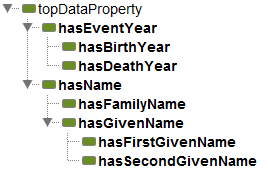
\includegraphics[width=\figwidth]{figures/new/event_name_hierarchy.PNG}\caption{The event year and name data property hierarchies in the \fhkb.}\label{fig:data_hierarchy}
\end{center}
\end{figure}

Do the following:
\steps{Data properties}{
\item Create the data properties as described in Figure~\ref{fig:data_hierarchy};
\item Give the \con{hasName} property the domain of \person and the range of \con{String};
\item Make the leaf properties of given names functional;
\item Add the names shown in Table~\ref{tab:familydata} (appendix); Again, it may be easier to read the names of the individual names.
\item Ask the questions:
\subitem all the people with the first given name `James';
\subitem all the people with the first given name `William';
\item All the people with the given name `William';
\item All the people with the given name `William' and the family name `Bright'.
}

The name data property hierarchy and the queries using those properties displays what now should be familiar.
Sub-properties that imply the super-property. So, when we ask \con{hasFirstGivenName value "William"} and then the query \con{hasGivenName value value "William"} we can expect different answers. There are people with `William' as either first or second given name and asking the question with the super-property for given names will collect both first and second given names.

\section{Summary}

We have used data properties that link objects to data such as string, integer, floats and Booleans etc. OWL uses the XML data types. We have seen a simple use of data properties to simulate birth years. The full \fhkb also uses them to place names (given and family) on individuals as strings. This means one can ask for the \person with the given name "James", of which there are many in the \fhkb.

Most importantly we have re-visited the open world assumption and its implications for querying an OWL ABox. We have looked at ways in which the ABox can be closed down -- unreliably via the functional characteristic (in this particular case) and more generally via type assertions.

All the DL queries used in this chapter can also serve as defined classes in the TBox. It is a useful exercise to progressively add more defined classes to the \fhkb TBox. Make more complex queries, make them into defined classes and inspect where they appear in the class hierarchy. 
\\
\expressivity{SROIQ(D)}

\ctime{1891157}{1134}{201}

\note{Note that we now cover the whole range of expressivity of OWL~2. HermiT at least is impossibly slow by now. This may be because HermiT does more work than the others. For now, we recommend to use either Pellet or FaCT++.}